%%%%%%%%%%%%%%%%%%%%%%% file template.tex %%%%%%%%%%%%%%%%%%%%%%%%%
%
% This is a general template file for the LaTeX package SVJour3
% for Springer journals.          Springer Heidelberg 2010/09/16
%
% Copy it to a new file with a new name and use it as the basis
% for your article. Delete % signs as needed.
%
% This template includes a few options for different layouts and
% content for various journals. Please consult a previous issue of
% your journal as needed.
%
%%%%%%%%%%%%%%%%%%%%%%%%%%%%%%%%%%%%%%%%%%%%%%%%%%%%%%%%%%%%%%%%%%%
%
% First comes an example EPS file -- just ignore it and
% proceed on the \documentclass line
% your LaTeX will extract the file if required
\begin{filecontents*}{example.eps}
%!PS-Adobe-3.0 EPSF-3.0
%%BoundingBox: 19 19 221 221
%%CreationDate: Mon Sep 29 1997
%%Creator: programmed by hand (JK)
%%EndComments
gsave
newpath
  20 20 moveto
  20 220 lineto
  220 220 lineto
  220 20 lineto
closepath
2 setlinewidth
gsave
  .4 setgray fill
grestore
stroke
grestore
\end{filecontents*}
%
\RequirePackage{fix-cm}
%
%\documentclass{svjour3}                     % onecolumn (standard format)
%\documentclass[smallcondensed]{svjour3}     % onecolumn (ditto)
\documentclass[twocolumn]{svjour3}       % onecolumn (second format)
%\documentclass[twocolumn]{svjour3}          % twocolumn
%
\smartqed  % flush right qed marks, e.g. at end of proof
%
\usepackage{color}
\usepackage[usenames,dvipsnames,svgnames,table]{xcolor}
\usepackage{booktabs}
\usepackage{tabu,xcolor,colortbl}
\usepackage{rotating}
\usepackage{amsmath,array}    
\usepackage[utf8]{inputenc} 
\DeclareUnicodeCharacter{FB01}{fi} %Caracter especial
\usepackage{graphicx} %Imagens
\usepackage{listings} % Codes
\usepackage{tabularx} % in the preamble
\usepackage{mathtools} % Serve para as equacoes

\usepackage{hyphenat}
\usepackage[english]{babel}
\hyphenation{ef-fect-ive consi-de-red demons-trate se-cond veri-fication covera-ge des-cribe reali-zation opera-tor re-pre-sentation methodo-lo-gy di-gi-tal chara-cteristics granu-lar ge-nerally diago-nal para-meters spe-cification re-presentable me-thods ope-rations sche-dule deve-loped des-cribes diffe-rent mo-dels sa-ving ve-rified proper-ties mini-mum mathe-matical tole-rated limi-ted op-tical net-works semi-conduc-tor go-to-pro-grams}

\newcommand{\head}[1]{\textnormal{\textbf{#1}}}
\renewcommand{\lstlistingname}{Algorithm}

\usepackage{color}
\definecolor{dkgreen}{rgb}{0,0.6,0}
\definecolor{gray}{rgb}{0.5,0.5,0.5}
\definecolor{mauve}{rgb}{0.58,0,0.82}
\definecolor{Gray}{gray}{0.93}
\definecolor{DarkGray}{gray}{0.70}

\lstset{frame=tb,
  language=c,
  aboveskip=3mm,
  belowskip=3mm,
  showstringspaces=false,
  columns=flexible,
  basicstyle={\small\ttfamily},
  numbers=none,
  numberstyle=\tiny\color{gray},
  keywordstyle=\color{black},
  commentstyle=\color{dkgreen},
  stringstyle=\color{mauve},
  breaklines=true,
  breakatwhitespace=true,
  tabsize=3
}
\DeclareGraphicsExtensions{.pdf,.png,.jpg}
%
% \usepackage{mathptmx}      % use Times fonts if available on your TeX system
%
% insert here the call for the packages your document requires
%\usepackage{latexsym}
% etc.
%
% please place your own definitions here and don't use \def but
% \newcommand{}{}
%
% Insert the name of "your journal" with
% \journalname{myjournal}
%

\begin{document}
\title{Applying Multi-Core Model Checking to Hardware-Software Partitioning in Embedded Systems}
\author{Alessandro Trindade\and Hussama Ismail\and Renato Degelo\and Edilson Galv\~ao\and Lucas Cordeiro}

\institute{A. Trindade, H. Ismail, R. Degelo, E. Galv\~ao \at
              Graduate Program in Electrical Engineering, Federal University of Amazonas, Brazil \\
%              Tel.: +123-45-678910\\
%              Fax: +123-45-678910\\
              \email{\{iurybessa, hussamaibrahim\}@ufam.edu.br and\\{\{rdegelo, esj.galvao\}@gmail.com}}          %  \\
%             \emph{Present address:} of F. Author  %  if needed
           \and
           L. Cordeiro \at
              Electronic and Information Research Center, Federal University of Amazonas, Brazil
              \email: lucascordeiro@ufam.edu.br           %  \\
}

\maketitle

\begin{abstract}
\textcolor{blue}{Atualizar o abstract para descrever brevemente os novos algoritmos desenvolvidos}
We present an alternative approach to solve the hardware (HW) and software (SW) partitioning problem, which uses Bounded Model Checking (BMC) based on Satisfiability Modulo Theories (SMT) in conjunction with a multi-core support using Open MultiProcessing. The multi-core SMT-based BMC approach allows initializing many verification instances based on processors cores numbers available to the model checker. Each instance checks for a different optimum value until the optimization problem is satisfied. The goal is to show that multi-core model-checking techniques can be effective, in particular cases, to find the optimal solution of the HW-SW partitioning problem using an SMT-based BMC approach. \textcolor{Red}{O problema de particionamento de HW-SW foi modelo em diversas plataformas como: MATLAB R2013a da MathWorks[19], Z3 um solucionador de teoremas da Microsoft Research[32] e ESBMC utilizando abordagens single-core e multi-core. Os algoritmos implementados são discutidos e suas particularidades destacadas, por fim, faz-se um comparativos dos resultados obtidos. }
\keywords{hardware-software co-design \and hardware-software partitioning\and optimization\and model checking\and multi-core\and OpenMP }
\end{abstract}

\section{Introduction}
Nowadays, with the strong development of embedded systems, the design phase plays an important role. At early stages, the design is split into separated flows: hardware and software. Consequently, the partitioning decision process, which deals with the decisions upon which parts of the application have to be designed in hardware (HW) and which in software (SW), must be supported by any well-structured methodology. If not, this leads to a number of issues (design flow interruptions, redesigns, and undesired iterations) which affects the overall development process, the quality and the lifecycle of the final system. Starting at the 1990s, intensive research was performed, and several approaches proposed, as shown in [1] and [2].

In any HW and SW design of complex systems, more time is spent on verification than on construction [3]. Formal methods based on model checking offer great potential to obtain a more effective and faster verification in the design process. Programs may be viewed as mathematical objects with behavior that is, in principle, well determined. This makes it possible to specify programs using mathematical logic, which constitutes the intended (correct) behavior. Then, one can try to give a formal proof or otherwise establish that the program meets its specification [4]. Research in formal methods has led to the development of very promising verification techniques, which facilitate the early detection of errors. Model-based verification techniques use models that describe the possible system behavior in a mathematically precise and unambiguous manner. The system models are accompanied by algorithms that systematically explore all the states of the system model.

In [5] and [6] was shown that it is possible to use Bounded Model Checking (BMC) based on Satisfiability Modulo Theories (SMT) to perform HW-SW partitioning in embedded systems. The present work extends those studies since there is a substantial improvement in terms of the genetic algorithm and the SMT-based verification method, which has been extended with a multi-core architecture. Multi-core processors have been used in all segments of industry to implement high-performance computing [7]. In particular, hardware platforms, together with multi-processing platforms, have allowed verification algorithms to distribute tasks executions across multiple processors, which generate an increase in performance if compared to single-core solution. However, most verification algorithms still disregard the limitations of the CMOS technology, which limits the increase of the chip’s frequency after it reaches 4 GHz.

\textcolor{blue}{Deve-se citar as referencias usando o comando cite do latex}

\textcolor{Red}{\textcolor{blue}{Descrever brevemente o funcionamento dos algortimos propostos} Here, we exploit the availability of multi-core processors; in particular, SMT-based verification methods applied to the HW-SW partition propose are proposed, then the results are compared using ILP (integral linear programming), GA (generic algorithms) in a multi-core version, and the vZ tool that is a state-of-art optimization tool [32].} 

\textcolor{Red}{O algoritmo ILP usa a intlinprog da biblioteca "Optimization Toolbox"[35], sua funcao é procurar o menor valor que satisfaca o problema descrito na Eq.(1). entretanto, para determinados tipos de problema ILP se torna inviavel dado o alto custo computacional, GA é uma forma de otimizar o tempo de processamento em detrimento da precisão, uma vez que GA não garante achar o valor máximo ou minimo para a problema. vZ usa funcoes de otimizacao e reescreve formulas em SMT para achar a solucao ideal, vZ apoia sua solucao em motores(OptSMT, MaxSMT).}

To the best of our knowledge, this is the first work to use a multi-core SMT-based verification to solve a HW-SW partitioning problem in embedded systems. We implement our ideas with the Efficient SMT-based Bounded Model Checker (ESBMC) tool [14]. As its main contribution, this paper shows that it is possible to take advantage of an SMT-based BMC tool in a multi-core architecture to solve optimization problems.

\textcolor{blue}{Voces precisam citar as secoes usando o comando ref do latex. Para isso, cada secao deve conter um label.}
\textcolor{Red}{This article is organized as follows: Section~\ref{background} gives a background on optimization, optimization with vZ, use of BMC technique with ESBMC, multi-cre ESBMC using OpenMP, ESBMC using optimized techniques of search to multiples cores with OpenMP. Section 3 describes the informal and formal mathematical modeling. Section 4 briefly describes th ILP and GA. The BMC method is based on SMT and is presented in section 5. The section 6 presents the paritioning model using vZ. The section 7 presents the experimental evaluation. The Section 8 discusses about the related works. Section 9 presents the conclusions and the future work.}

%----------------------------------------------
\section{Background}
\label{background}
%----------------------------------------------

\textcolor{blue}{Introduzir uma breve descrição da seção.}

\textcolor{red}{Optimization is the act of obtaining the best result (i.e., the optimal solution) under given circumstances [9]. In the design, construction, and maintenance of any engineering system, engineers have to make many technological and managerial decisions at several stages. The ultimate goal of all such decisions is either to minimize the effort required or to maximize the desired benefit. Because the effort required or the benefit desired in any practical situation can be expressed as a function of certain decision variables, optimization can be defined as the process of finding the conditions that give the maximum or minimum value of a function [9].}
%----------------------------------------------
\subsection{Optimization}
%----------------------------------------------

There is no single method available for solving all optimization problems efficiently [9]. The most known technique is linear programming, which is an method applicable for the solution of problems in which the objective function and the constraints appear as linear functions of the decision variables. A particular case of linear programming is ILP, in which the variables can assume just integer values. Eq. (1) shows a typical linear programming problem, where  and  are vectors or matrixes that describe the constraints
\begin{equation}
  minf^t x \: such that  = 
  \begin{cases}
    A.x \leq b, \\ 
    Aeq.x = beq, \\ 
    x \geq 0.
  \end{cases}
\end{equation}

In some cases, the time to find a solution using ILP is impractical. Even with the use of powerful computers, a problem can take hours belerunning before an optimal solution is reached. If the optimization problem is complex, some heuristics can be used to solve the same problem faster, e.g., those used in the GA [9]. The only drawback is that the found solution may not be the global minimum or maximum.

\textcolor{red}{Ferramentas como vZ e ESBMC tambem exploram o problema de otimizacao, ambas ferramentas tem como principal finalidade a precisão na resposta, problemas com uma quantidade muito grande de dados torna o tempo um impecilho. as secoes 2.2 e 2.3 demonstram como vZ e ESBMC usam respectivamente suas tecnicas para resolucao dos problemas de particionamento, espera-se destas tecnicas uma resposta exata em um tempo razoavel.}


%----------------------------------------------
\subsection{\textcolor{Red}{Optimization with Vz}}
%----------------------------------------------

A SMT solver is a tool that verifies formula's satisfiability based in a set of rules SMT. Z3 is a SMT solver made by Microsoft Research, freely available to the community, that supports a variety of theories. Z3 brings a solver DPLL together with a correspondence machine for quantifiers. Z3 is implemented in C++.
vZ is one of the tools implemented on the Z3 solver, it's base function is to optimize objectives within the logic context of constraints, it stands for the functions that make possible formulate optimized criteria.
vZ includes an incremental version of MaxRes to MaxSAT and a Simplex to solve numbers without defined patterns, in it's core MaxSAT is responsible to the restrictions while OptSMT optimize the linear arithmetic objectives.
Among all progress of Z3 using vZ the functions hightlights: maximize, minimize e assert-soft.

\begin{itemize}
\item{\textbf{maximize(T)}
this instruction informs to the solver that a given variable T should be maximized, if possible maximize real, integer and bit vector values.}
\item{\textbf{minimize(T)}
this instruction informs the solver that a given variable T should be minimized, the accepted types are the same as maximize.}
\item{\textbf{Assert-Soft F :weight n}
the instruction Asser-soft is a restriction to F, if possible add a weight n, the default is 1.}
\end{itemize}

Lets optimize (K+W), with the restrictions in (K \textless 2) and (W-K \textless 1), the expected result of the optimization described in the code below is 2. the model generated by vZ shows that K = 1 and W = 1.

\begin{lstlisting}[caption=Code "SMT" using vZ, label=vZ]
1. (declare-const K Int) 
2. (declare-const W Int)
3. (assert (< K 2)) 
4. (assert (< (- W K) 1))
5. (maximize (+ K W)) 
6. (check-sat)
\end{lstlisting}


Accordingly to [34] the architecture of vZ can be described on the image XXX, initially the formulas and the SMT objectives are converted to problems MaxSAT, if there are many objectives, vZ invokes MaxSAT or OptSAT. To restrictions in real values using “Box”, vZ combines all linear arithmetic and calls the OptSMT. When we use “soft constrains” in the mode “lexicographic” vZ invokes MaxSAT.
\begin{figure}[ht]
	\centering
  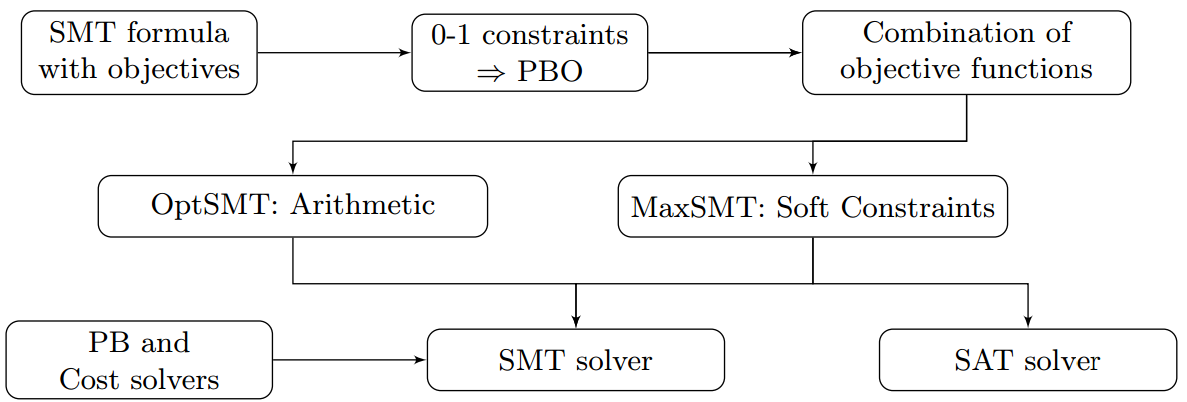
\includegraphics[width=0.49\textwidth, height=95px]{Image/vzArch.png} 
	\caption{vZ Architecture}
	\label{fig2}
\end{figure}

Z3 is available for platforms like C, C ++, Java, .NET and Python, it is possible to download the Z3 with vZ in http://z3.codeplex.com. API in python was used to formulate the optimization problem on the vZ tool. 

%----------------------------------------------
\subsection{Bounded Model Checking with ESBMC}
%----------------------------------------------

Model checking refers to algorithms for exploring the state space of a transition system to determine if it obeys a specification of its intended behavior [3], [4]. These algorithms can perform exhaustive exploration in a highly automatic way and, thus, have attracted much interest in industry. However, model-checking has been held back by the state explosion problem, in which the number of states in a system grows exponentially in the number of system components [10]. Much research has been devoted to mitigate this problem.

Among the recent techniques, there is one that combines model checking with satisfiability solving. This technique, known as bounded model checking (BMC), does a very fast exploration of the state space, and for some types of problems, it offers large performance improvements over previous approaches, as shown in [10]. In particular, BMC based on Boolean Satisfiability (SAT) has been introduced as a complementary technique to binary decision diagrams for alleviating the state explosion problem. 

The basic idea of BMC is to check the negation of a given property at a given depth: given a transition system $ M $, a property $ \phi $, and a bound $ K $, BMC unrolls the system  times and translates it into a verification condition (VC) $ \varphi $  such that $ \varphi $   is satisfiable if and only if $ \phi $ has a counterexample of depth $ K $ or less [10]. To cope with increasing software complexity, SMT solvers can be used as back-ends for solving the generated VCs, as shown in [11], [12], and [13]. 

According to [14] and [15], SMT-based model checking can be used to verify the single- and multi-threaded software. In [16], ESBMC can also be used to model check C++ software based on SMT solvers. In [5] and [6] it was shown that it is possible to use ESBMC, as an optimization tool.

There are two directives in C/C++ that can be used to guide a model checker to solve an optimization problem: ASSUME and ASSERT. The directive ASSUME is responsible for ensuring the compliance of constraints (software costs), and the directive ASSERT controls the halt condition or code violation (minimum hardware cost). Then, with some C/C++ code, it is possible to guide ESBMC to solve optimization problems.


%----------------------------------------------
\section{Mathematical modeling}
%----------------------------------------------

The mathematical modeling was taken from [1], [2].

%----------------------------------------------
\subsection{Informal Model (or Assumptions)}
%----------------------------------------------

The informal model can be described by five characteristics. First, there is only one software context, i.e., there is just one general-purpose processor, and there is only one hardware context. The components of the system must be mapped to either one of these two contexts. Second, the software implementation of a component is associated with a software cost, which is the running time of the component. Third, the hardware implementation of a component has a hardware cost, which can be area, heat dissipation, and energy consumption. Fourth, based on the premise that hardware is significantly faster than software, the running time of the components in hardware is considered as zero. Finally, if two components are mapped to the same context, then there is no overhead of communication between them; otherwise, there is an overhead. The consequence of these assumptions is that scheduling does not need to be addressed in this work. Hardware components do not need scheduling, because the running time is assumed to be zero. Because there is only one processor, software components do not need to be scheduled as well. Therefore, the focus is only on the partitioning problem. That configuration describes a first-generation co-design, where the focus is on bipartitioning [17].

%----------------------------------------------
\subsection{Formal Model}
%----------------------------------------------

The inputs of the problem are: A directed simple graph $ G = (V,E) $, called the task graph of the system, is necessary. The vertices $ V = \{V_1,V_2,\dotso,V_n\} $ represent the nodes that are the components of the system that will be partitioned. The edges $ E $ represent communication between the components. Additionally, each node  $ V_i $ has a cost $ h(V_i) $ (or $ h_i $ of hardware (if implemented in hardware) and a cost $ s(s_i) $ (or $ s_i $ of software (if implemented in software). Finally, $ c(V_i,V_j) $ represents the communication cost between $ V_i $ and $ V_j $ if they are implemented in different contexts (hardware or software).

Based on [1],  is called a hardware-software partition if it is a bipartition of $ V:P = (V_h, V_s) $ , where $ V_h \cup V_s = V $  and $ V_h \cap V_s = 0$  . The crossing $ E_p = \{(V_i,V_j):V_i \in V_s, V_j \in V_h \;or\; v_i \in V_h, v_j \in V_s $ edges are . The hardware cost of $ P $  is given by Eq. (2), and the software cost of $ P $ (i.e., software cost of the nodes and the communication cost) is given by Eq. (3):

\begin{align}
\ H_p &= \Sigma (v_i \;\in\; _Vh) H_i\\
  S_p &= \Sigma (v_i \;\in\; _Vs) S_i + \Sigma (_(v_i,v_j) \in\; _Ep)\; C(V_i, V_j)
\end{align}

Three different optimization and decision problems can be defined. In this paper, the focus is on the case that $ S_0 $ is given, i.e., to find a $ P $ HW-SW partitioning so that $ S_p \leq S_0 $ and $ H_p $ is minimal (system with hard real-time constraints). So, based on Eq. (1) and Eq. (3) the optimization problem’s restrictions can be reformulated as: $ s(1-x) + c|E_x| \leq S_0 $, where $ x $ is the decision variable. Concerning the complexity of this problem, reference [1] demonstrates that it is NP-Hard.

%----------------------------------------------
\section{Partitioning problem using ILP-based,Genetic Algorithms}
\label{ILPGA}
%----------------------------------------------

The ILP and GA were taken from [5] and [6]. Both use slack variables in order to be possible to represent the constraints and to use commercial tools. However, GA had improvements from the parameters of related studies in order to increase the solution accuracy without producing timeout. The tuning was performed by empirical tests and resulted in changing of three parameters, which are passed to function ga of MATLAB [18]: the population size was set from 300 to 500, the Elite count changed from 2 (default value) to 50, and the number of Generations changed from 100* NumberOfVariables (default) to 75.

%----------------------------------------------
\section{Analysis of the partitioning problem using ESBMC}
%----------------------------------------------

\textcolor{blue}{Introducao da secao.}

%----------------------------------------------
\subsection{Multi-core ESBMC with OpenMP}
%----------------------------------------------

Nowadays, although the CPU used to perform tests usually has a modern multi-core architecture, with the ability to run several threads on different processing cores, ESBMC verification runs are still performed only in a single-core. For instance, if the processor has 8 processing cores available, only one is used for the verification and the others remain idle. There is a significant unused hardware resource during this process.

Fig.1 shows the ESBMC architecture, which consists of the C/C++ parser, GOTO Program, GOTO Symex, and SMT solver [16]. In particular, ESBMC compiles the C/C++ code into equivalent GOTO\hyp{}programs (i.e., control-flow graphs) using a gcc-compliant style. The GOTO-programs can then be processed by the symbolic execution engine, called GOTO Symex, where two recursive functions compute the constraints ($ C $) and properties ($ P $); finally it generates two sets of equations (i.e.,\:$ C \land \neg P $ ) which are checked by an SMT solver. 

The main factor for ESBMC to use only a single-core relies on its back-end (i.e., SMT Solver). Currently, the SMT solvers supported by ESBMC are: Z3 [24], Boolector [25], MathSAT [26], CVC4 [27], and Yices [28]. Most of them do provide neither multi-threaded support nor a parallel version to solve the generated SMT equations.
\begin{figure}[ht]
	\centering
  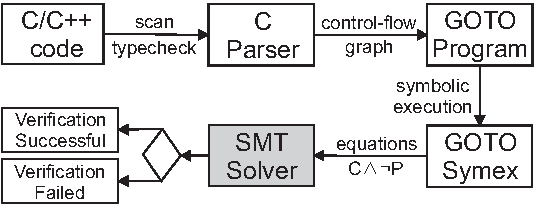
\includegraphics[scale=0.9]{Image/esbmc-arch-new.pdf} 
	\caption{gestaucht}
\end{figure}

To optimize the CPU resources utilization without modifying the underlying SMT Solver, the Open Multi-Processing (OpenMP) library [23] is used in this present work as a front-end for ESBMC.

OpenMP is a standard Application Programming Interface (API) for shared memory programming, which has been very successful for structural parallelism in applications. The API provides a directive-based programming approach to write parallel versions of C/C++ programs [33]. In OpenMP, the implementation is based on the fork-join model. The main thread executes the sequential parts of the program; if a parallel region is encountered, then it forks a team of worker threads. After the parallel region finishes (i.e., the API waits until all threads terminate), then the main procedure gets back to the single-threaded execution mode [7]. Fig. 2 shows our approach called “Multi-core ESBMC”.
\begin{figure}[ht]
	\centering
  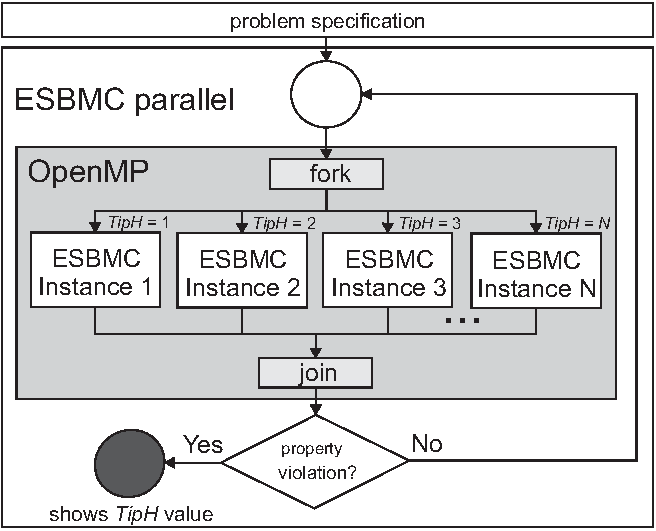
\includegraphics[scale=0.75]{Image/esbmc-parallel.pdf} 
	\caption{gestaucht}
\end{figure}

Multi-core ESBMC obtains the problem specification represented by a C program, which is violated when the correct optimum value () parameter is reached; Multi-core ESBMC starts a parallel region with  different instances of ESBMC, based on the number of available processing cores. All these ESBMC instances run independently of each other, as shown in Fig. 2; note that there is no shared-memory (or message-passing) mechanism among the threads. In particular, different threads are managed by the OpenMP API, which is responsible for the thread lifecycle: start, running, and dead states, using different  values as condition. After executing  instances, if there is no code violation, then multi-core ESBMC starts  new instances again. During the parallel region execution, if a violation is found in any running thread, then it presents the counterexample with the violation condition and the verification time. If all threads of the batch processing are terminated, then multi-core ESBMC finishes its execution.

%----------------------------------------------
\subsection{\textcolor{Red}{Multi-core ESBMC with OpenMP using Binary Search}}
%----------------------------------------------

\textcolor{Red}{The original parallelization was made by continuously forking the instances of the ESBMC until the first violation is find. Since OpenMP only returns from a parallelized loop when every forked thread finishes, some processor could remain idle for some time.}

\begin{figure}[ht]
	\centering
  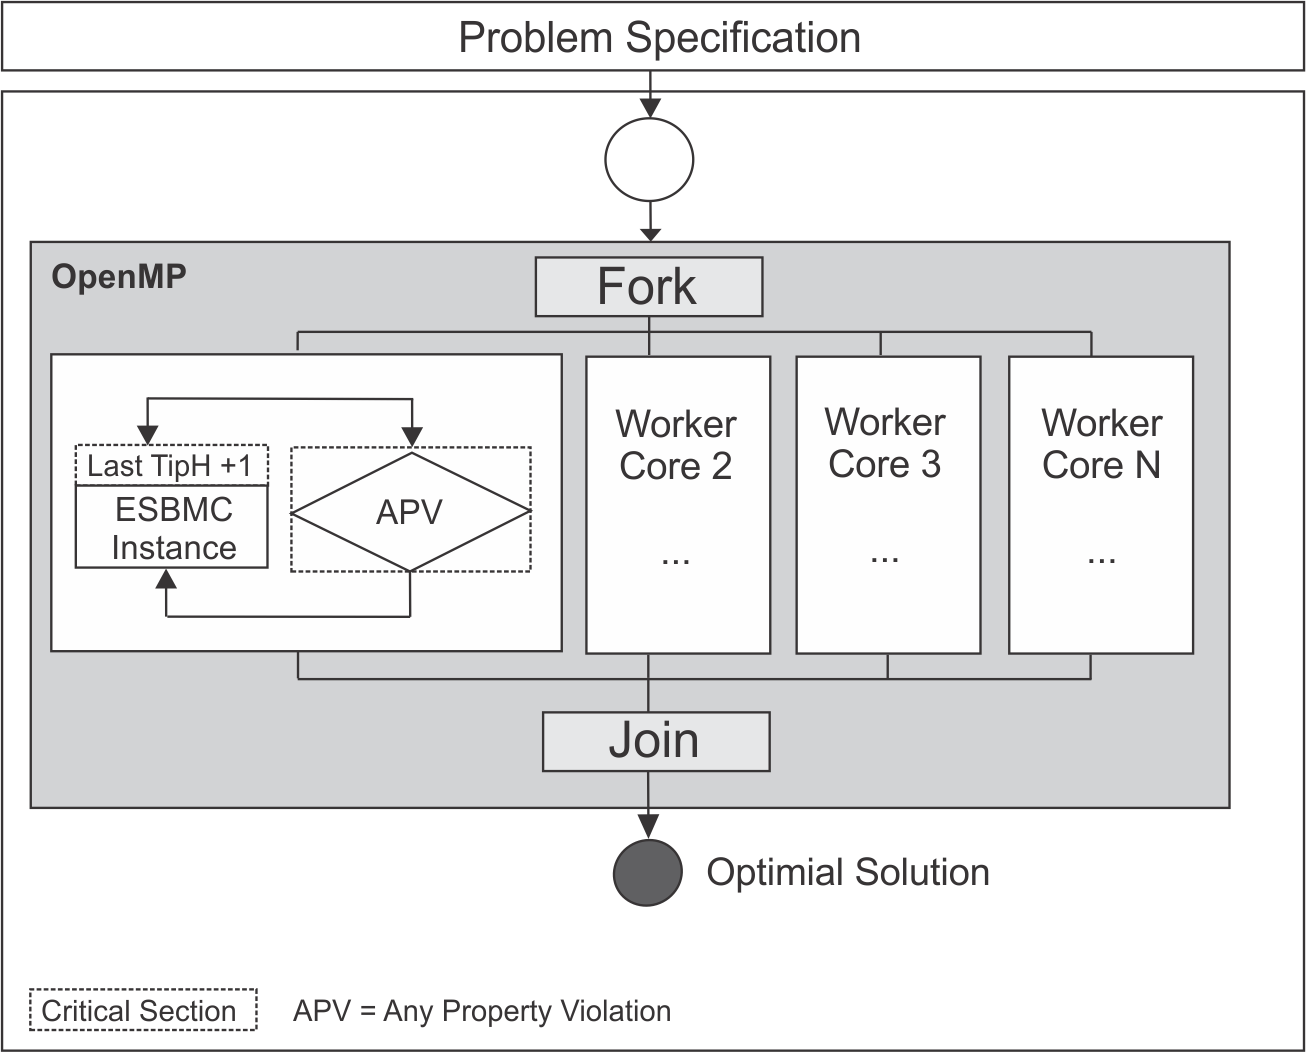
\includegraphics[scale=0.75]{Image/esbmc-parallel.png} 
	\caption{gestaucht}
	\label{fig2}
\end{figure}

\textcolor{Red}{Consequently, the first approach aims to remove the idle time from the parallel loops, by creating workers inside the threads to execute the next step until a violation is found. This approach could potentially lead to a great improvement, but as ESBMC executes the sequential steps almost at the same time, the processor does not remain idle for a longer period and thus there is almost no optimization.}

\textcolor{Red}{The most optimized approach applies a parallelized binary search to reduce the amount of steps executed  in order to find the most optmized solution. As a result, the controller is designed to return the best step to execute so that the number of steps are reduced as maximum as possible. The parallelized binary search accomplishes this by splitting the domain into intervals and then returning the middle of the largest interval, which thus creates two new intervals.}
\begin{figure}[ht]
	\centering
  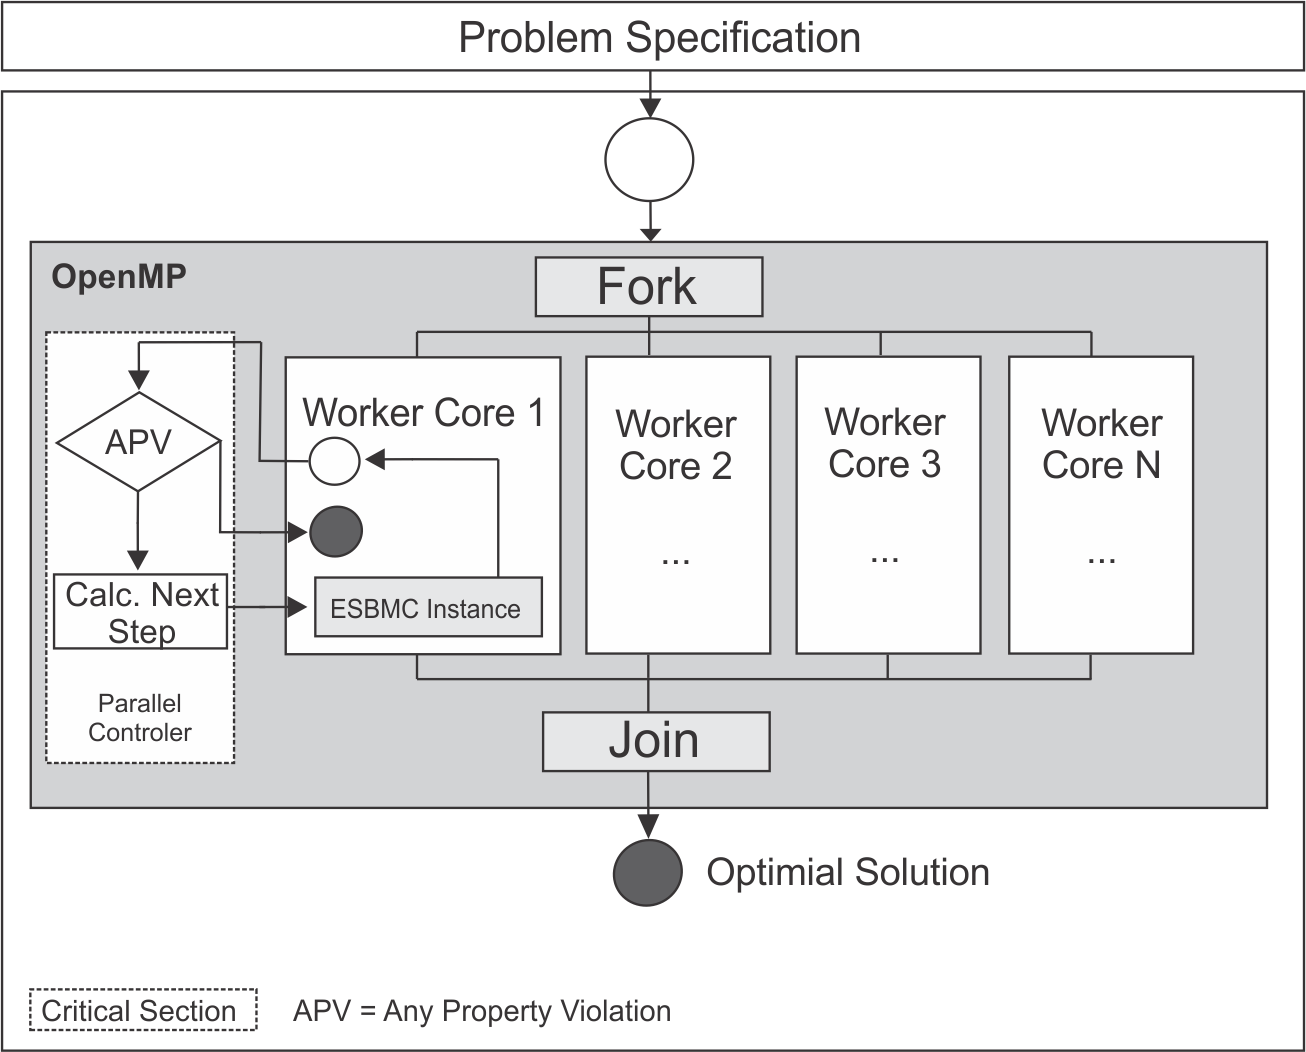
\includegraphics[scale=0.75]{Image/esbmc-parallel-Controler.png} 
	\caption{gestaucht}
	\label{fig2}
\end{figure}

\textcolor{Red}{As example, given a problem of domain 1 to 20, firstly we create an initial interval from 1 to 20. When the next available core asks for a step to execute, the controller gets the biggest interval, which in this case is 1 – 20, divide it by 2, creates two new intervals and return the middle of the original interval. Therefore, there would be 2 new intervals, one from 1 to 9 and another one from 11 to 20, and the returned step would be 10. The controller also checks when an interval has less than two elements to avoid the creation of empty or invalid intervals. }
\begin{figure}[ht]
	\centering
  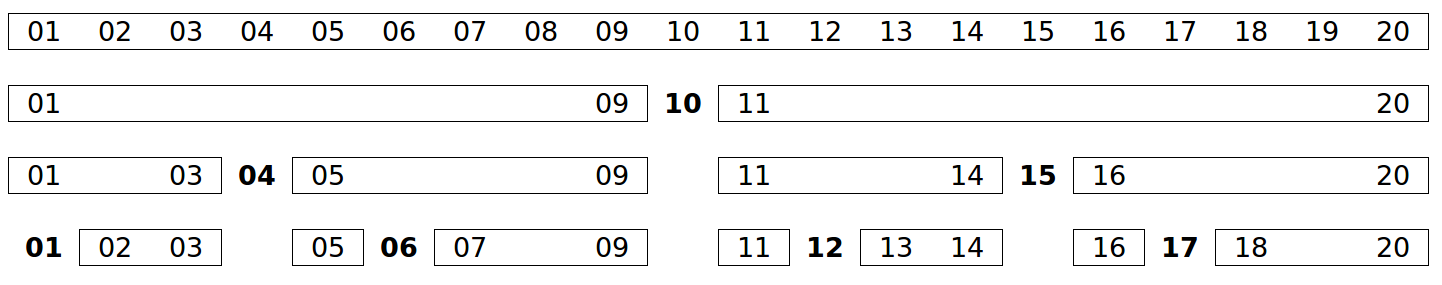
\includegraphics[width=0.49\textwidth, height=75px]{Image/Fig4.png}
	\caption{gestaucht}
	\label{fig2}
\end{figure}

\textcolor{Red}{Additionally, since there is a gap between the steps, produced by the customized binary search; in particular, there might be several steps are not executed. For instance, in the example above, if step 10 returns false, then one can conclude that all steps after 10 is false as well. However, if the same step 10 is true, we can assume that all steps before 10 is true as well.}

\textcolor{Red}{As a result, a method to remove unnecessary steps is implemented in the controller by removing or shrinking existing intervals. This approach leads to a high impact in the verification time. However, if a step is running and is not needed anymore, the worker kills the forked process and starts a new one.}

\textcolor{blue}{Colocar um caption em todos os algoritmos.}

\begin{lstlisting}[caption=Calculate Steps and Chunks]
01. GetNextStep(){
02.  int largestChunk = -1;
03.  chunk largest;
04.  for each(chunk in chunks){
05.     if(chunk.right - chunk.left > largestChunk){
06.           largestChunk = chunk.right - chunk.left;
07.           largest = chunk;
08.     }
09.   }	
10.   chunks.remove(largest);	
11.   int median = largest.left + floor((largest.right - largest.left) / 2)
12.   if(median > 0){
13.      if(largest.right - largest.left > 1)
14.         chunks.add(new chunk(largest.left, median - 1));	
15.      if(largest.right != largest.left)
16.         chunks.add(new chunk(median + 1, largest.right);
17.    }
18.   return median;
19. }
\end{lstlisting}
\textcolor{Red}{The algorithm above describes how the customized binary search calculates and returns the step to be executed. From line 4 to 9 the algorithm finds the biggest interval. Then from the line 10 the biggest interval is removed and the median is calculated in the line 11. Then 2 new intervals are created, the left side on line 14 and the right side on the line 16. At the end, the median is returned.}

\textcolor{blue}{Colocar um caption em todos os algoritmos.}

\begin{lstlisting}[caption=Manager Controller]
01. step = controller.GetNextStep();
02. int pid = ExecuteStep(step);
03. while(isRunning(pid)){
04.   if(!controller.isNeeded(step))
05.    kill(pid);
06. }     
\end{lstlisting}
\textcolor{Red}{The algorithm above describes how the worker starts and monitors the ESBMC instances. The algorithm starts by retrieving the step to execute from the controller (line 1) , starts the instance of ESBMC and get the process id from the forked process (line 2). While the step is being executed, the controller checks whether this step is still needed (line 4). If not, then the ESBMC instance is killed (line 5) and the worker is free to initiate another step.}

%----------------------------------------------
\section{Verification Algorithm using ESBMC}
%----------------------------------------------

ESBMC pseudocode shows the algorithm with the same restrictions and conditions placed on ILP and GA. Two values must be controlled to obtain the results and to perform the optimization. One is the initial software cost, as defined in Section III.G. The other is the halting condition (code violation) that stops the algorithm.

The ESBMC algorithm starts with the declarations of hardware, software, and communication costs.  also must be defined, as the transposed incidence matrix and the identity matrix, as typically done in MATLAB. Here, the matrices A and b are generated. At that point, the ESBMC algorithm starts to differ from the ILP and GA presented in [5] and [6].

It is possible to tell the ESBMC with which type of values the variables must be tested. Therefore, there is a declaration to populate all the decision variables $ x $ with non-deterministic Boolean values. Those values that change for each test will generate a possible solution and obey the restrictions. If this is achieved, then a feasible solution is found and the ASSUME directive is responsible for ensuring the compliance of constrains (i.e.,$ A.x \leq b $ ).

A loop controls the cost of hardware hint, starting with zero and reaching the maximum value considering the case, where all nodes are partitioned to hardware. To every test performed, the hardware hint is compared to the feasible solution. This is accomplished by an ASSERT statement at the end of the algorithm, a predicate that controls the halt condition (true-false statement). If the predicate is FALSE, then the optimization is finished, i.e., the solution was found. The ASSERT statement tests the objective function, i.e., the hardware cost, and will stop if the hardware cost found is lower than or equal to the optimal solution. However, if ASSERT returns a TRUE condition, i.e., the hardware cost is higher than the optimal solution, then the model-checking algorithm restarts and a new possible solution is generated and tested until the ASSERT generates a FALSE condition. When the FALSE condition happens at verification-time, the execution code is aborted and ESBMC presents the counterexample that caused the condition to be broken. That is the point in which the solution is presented (minimum HW cost).

In the ESBMC algorithm, which is shown below, it is not necessary to add slack variables because the modulus operation is kept, which reduces the number of variables to be solved. 

\textcolor{blue}{Colocar um caption em todos os algoritmos.}

\begin{lstlisting}[caption=Pseudocode describing ESBMC]
01. Initialize Variables 
02. Declare number of nodes and edges
03. Declare hardware cost of each node as array (h)
04. Declare software cost of each node as array (s)
05. Declare communication cost of each edge (c)
06. Declare the initial software cost of (S0)
07. Declare transposed incidence matrix graph G (E)
08. Define the solutions variable (Xi) as Boolean
09. main {
10.  for TipH = 0 to Hmax do {
11.   populate Xi with nondeterministic/test values
12.   Calculate s(1-x)+c|Ex| and store at variable
13.   Requirement isured by Assume (Variable <= S0)
14.   Calculate Hp cost Based on value tested of Xi
15.   Violation check with Assert(Hp > TipH)
16.  }
17. }
\end{lstlisting}

In the multi-core ESBMC algorithm, the only difference is the fact that the value of $ TipH $ and its range is not declared in the algorithm, as shown in ESBMC Pseudocode. The proposed approach is invoked for each test problem, as follows:
$ esbmc-parallel <Filename.c> \; <hminvalue> \; <Hmax> $

Where $ <Filename.c> $ is the optimization problem described in ANSI-C format, $  <hminvalue> $ is the minimum (zero to HW-SW partitioning problem) and $ <Hmax> $ is the maximum hardware cost for the specified problem.

Therefore, the algorithm starts  different instances of ESBMC using the different optimization values, in ascending order, for $ Hmax $ in order to find a violation. If all instances finish and no violation is found, then multi-core ESBMC starts new $ N $ instances. When a violation is found, it reports time and hardware cost. If multi-core ESBMC tests all the possibilities for the hardware cost and has not found a violation, then it reports: $ Violation not found $.

%----------------------------------------------
\section{\textcolor{Red}{Analysis of the partitioning problem using vZ}}
%----------------------------------------------

The code below shows the conditions applied on ILP, GA and ESBMC converted to the vZ tool described in [34] and [35]. 

A vZ context is created, it receives the restrictions and returns the model if a solution to the set of rectictions exists. Later the number of nodes are declared, number of edges, the number of, the cost of hardware, cost of software, cost of communication and the incidence matrix E.

The arithmetic declarations described on the lines 10, 11,12 e 13 of the code are a transcription of the formula $ S(1-x) + C|Ex| \leq S{0} $ described on the section III.B, refers to the cost of software (SF). Note that in the line 11 a temporary variable called TMP is created to represent $C|Ex|$  , then the product between the absolute value of TMP and the vector C declared in the line 07, then the result of the cost of communication is generated (CMC). 

In the line 13, the Fobj (Objective Function) is declared. It is a product between the cost of hardware with the vector that contains the values 0 and 1. Fobj should be minimized to get the best hardware solution .

Two restrictions are imposed, the first refers to the sum between the cost of software and communication, the result of the sum should be less than , the second restriction tells to vZ that Fobj should be minimized. So the model is checked, once a solution that complains the restrictions, the value of the Fobj is printed.

\textcolor{blue}{Colocar um caption em todos os algoritmos.}

\begin{lstlisting}[caption=Pseudocode describing vZ]
01.#Init Values
02.  Create vZ context 
03.  Create binary vector (x)
04.  Declare number of nodes, edges and S0
05.  Declare hardware cost of each node as array (h) 
06.  Declare software cost of each node as array (s)
07.  Declare communication cost of each edge (c)
08.  Declare transposed incidence matrix graph G (E)
09.#Arithmetic
10.  SF receive s(1-x)
11.  TMP vector receive E|x| 
12.  CMC receive c*|EX|
13.  Fobj receive  x[i] * h[i]
14.#Asserts
15.  Add restrictions (SF + CMC <= S0)
16.  Add restrictions to minimize Fobj
17.  Check Model
18.  Print Result
\end{lstlisting}

Nice team.

%----------------------------------------------
\section{Experimental Evaluation}
%----------------------------------------------

ESBMC 1.24 running on a 64-bit Ubuntu 14.04.1 LTS operating system was used. Version 2.0.1 of Boolector SMT-solver [25] (freely available) was used as well. For the ILP and GA formulations, MATLAB R2013a from MathWorks with Parallel Computing Toolbox was used [18]. MATLAB is a dynamically typed high-level language known as the state-of-the-art mathematical software [19] and is widely used by the engineering community [20]. \textcolor{Red}{The built in Z3 tool vZ [34] available freely was also used. A parallel approach of the ESBMC sequential search ascending, descending and binary was implemented in c++11}. A desktop with 24GB of RAM and i7 (8-cores) from Intel with clock of 3.40 GHz was used. Each time was measured 3 times in GA (average taken) and just once in ESBMC and ILP. The reason is that GA times are not so close as ESBMC and ILP. A time out condition (TO) is reached when the running time is longer than 7,200 seconds. A memory out (MO) occurs when the tool reaches 24GB of memory. TABLE I. lists the benchmarks1.

\begin{table}[h]
\caption {Description of Benchmarks}
\small
\sffamily\footnotesize
\tabulinesep=6pt
\begin{tabular}[c]{m{1.5cm}m{0.8cm}m{0.8cm}m{3.8cm}}
  \toprule[1.5pt]
  \head{Name} & \head{Nodes} & \head{Edges} & \head{Description}\\
  \midrule
  
\verb|CRC32| & \verb|25| & \verb|32| & \rmfamily 32-bit cyclic redundancy check [21]\\
\hline
\verb|Patricia| & \verb|21| & \verb|48| & \rmfamily Routine to insert values in Patricia Tree [21]\\
\hline

\verb|Dijkstra| & \verb|26| & \verb|69| & \rmfamily Computer shortest paths in a graph [21]\\
\hline
\verb|Clustering| & \verb|150| & \verb|331| & \rmfamily Image segmentation algorithm in a medical application\\
\hline
\verb|RC6| & \verb|329| & \verb|448| & \rmfamily RC6 cryptography graph algorithm\\
\hline
\verb|Fuzzy| & \verb|261| & \verb|422| & \rmfamily Clustering algorithm based on fuzzy logic\\
\hline
\verb|Mars| & \verb|417| & \verb|600| & \rmfamily MARS cipher from IBM algorithm\\
 
  \bottomrule[1.5pt]
\end{tabular}
\end{table}

\textcolor{Red}{The results obtained that standout were the ILP and vZ.
Vz solved correctly 4 of 7 algorithms, got an false positive in the algorithm RC6, the slowest result compared with ILP was Patricia that was 3.33 times faster, vZ returned two TO (time outs) in Fuzzy and Mars.}

\textcolor{Red}{In contrast, ILP solved correctly 6 of 7 algorithms, do not had any false positive, the resolution time is bigger compared with vZ and lower compared with ESBMC, it shows that ILP is optimized to solve problems but has an average resolution time.}

\textcolor{Red}{The only technique aqble to solve all algorithms was GA, however it's precision was not satisfatory, it had error rate between -37.6\% and 29.0\%.}

\textcolor{Red}{All versions of parallel ESBMC got better results compared with the sequential approach, stands out the binary version described on the section 2.5, the performance get better as the number of nodes and edges get bigger. The clustering algorithm when processed by the parallel ESBMC had 3.13 better performance than ILP, it`s time was 207 seconds and is very cloe to the solution of vZ that is 109 seconds.}

\textcolor{Red}{The table 2 shows the advances in the parallelization of algorithms of partitioning problems, ESBMC had great results when executed in parallel, the vZ and ILP had precise results as ESBMC.} 

\begin{table}[h]
\caption {Results of the benchmarks}
\small
\begin{tabular}[c]{m{1.3cm}m{1.20cm}|m{0.85cm}|m{0.85cm}|m{0.85cm}|m{0.85cm}}
  \toprule[1.5pt]
  \head{\begin{turn}{-90}  \end{turn}} &
  \head{\begin{turn}{-90}  \end{turn}} &
  \head{\begin{turn}{-90}CRC32\end{turn}} &
  \head{\begin{turn}{-90}Patricia\end{turn}} &
  \head{\begin{turn}{-90}Dijkstra\end{turn}} &
  \head{\begin{turn}{-90}Clustering\end{turn}} \\

  \midrule

\verb| | & \verb|Nodes| & \verb|25| & \verb|21| & \verb|26| & \verb|150| \\
\verb| | &\verb|Edges| & \verb|32| & \verb|48| & \verb|69| & \verb|331| \\
\verb| | &\verb|S0| & \verb|20| & \verb|10| & \verb|20| & \verb|50| \\
\bottomrule[1.5pt]

%EXACT Solution
\rowcolor{DarkGray}
\verb|Exact| & \verb|Hp| & \verb|15| & \verb|47| & \verb|31| & \verb|241| \\
\rowcolor{DarkGray}
\verb|Solution| & \verb|Sp| & \verb|19| & \verb|4| & \verb|19| & \verb|46| \\


%vZ
\verb|vZ| & \verb|T(s)| & \verb|0.2| & \verb|0.3| & \verb|0.6| & \verb|109|\\
\verb|| & \verb|Hp| & \verb|15| & \verb|47| & \verb|31| & \verb|241| \\
\hline

%ILP
\rowcolor{Gray}
\verb|ILP| & \verb|T(s)| & \verb|2| & \verb|1| & \verb|2| & \verb|649|\\
\rowcolor{Gray}
\verb| | & \verb|Hp| & \verb|15| & \verb|47| & \verb|31| & \verb|241|\\
\hline

%GA
\verb|GA| & \verb|T(s)| & \verb|7| & \verb|7| & \verb|9| & \verb|340|\\
\verb| | & \verb|E%| & \verb|13.3| & \verb|0| & \verb|29| & \verb|1.7|\\
\hline

%ESBMC
\rowcolor{Gray}
\verb|ESBMC| & \verb|T(s)| & \verb|31| & \verb|362| & \verb|292| & \verb|3010|\\
\rowcolor{Gray}
\verb|| & \verb|Hp| & \verb|15| & \verb|47| & \verb|31| & \verb|241|\\
\hline

%MultiCore ESBMC
\verb|ESBMC| & \verb|T(s)| & \verb|2| & \verb|6| & \verb|7| & \verb|1615|\\
\verb|MC| & \verb|Hp| & \verb|15| & \verb|47| & \verb|31| & \verb|241|\\
\hline

%ESBMC Parallel sequential
\rowcolor{Gray}
\verb|ESBMC| & \verb|T(s)| & \verb|4| & \verb|10| & \verb|11| & \verb|2238|\\
\rowcolor{Gray}
\verb|PS| & \verb|Hp| & \verb|15| & \verb|47| & \verb|31| & \verb|241|\\
\hline

%ESBMC Parallel Binary
\verb|ESBMC| & \verb|T(s)| & \verb|6| & \verb|5| & \verb|6| & \verb|207|\\
\verb|PB| & \verb|Hp| & \verb|15| & \verb|47| & \verb|38| & \verb|241|\\
\bottomrule[1.5pt]

\end{tabular}
\end{table}

\textcolor{Red}{A tabela 3 é uma extensão da tabela 2. A tabela 3 mostra problemas com uma quantidade maior de nós e arestas, este aumento impacta diretamente no tempo de processamento. RC6 obteve time out para todas as versões do ESBMC, vZ e GA não obtiveram resposta correta, e ILP resolveu corretamente o problema. Fuzzy teve 3 time outs, 3 memory outs, e uma resposta incorreta. ILP foi o unico que conseguiu resolver Mars, GA respondeu incorretamente e todos os outros algoritmos deram TO ou MO.  } 

\begin{table}[h]
\caption {Results of the benchmarks}
\small
\begin{tabular}[c]{m{1.3cm}m{1.25cm}|m{1.25cm}|m{1.25cm}|m{1.25cm}}
  \toprule[1.5pt]
  \head{\begin{turn}{-90}  \end{turn}} &
  \head{\begin{turn}{-90}  \end{turn}} &
  \head{\begin{turn}{-90}RC6\end{turn}} &
  \head{\begin{turn}{-90}Fuzzy\end{turn}} &
  \head{\begin{turn}{-90}Mars\end{turn}} \\

  \midrule

\verb| | & \verb|Nodes| & \verb|329| & \verb|261|  & \verb|417|\\
\verb| | &\verb|Edges| &  \verb|448| & \verb|442|  & \verb|600|\\
\verb| | &\verb|S0| & \verb|600| & \verb|4578|  & \verb|300|\\
\bottomrule[1.5pt]

%EXACT Solution
\rowcolor{DarkGray}
\verb|Exact| & \verb|Hp| & \verb|692|  & \verb|13820| & \verb|876|\\
\rowcolor{DarkGray}
\verb|Solution| & \verb|Sp| & \verb|533|  & \verb|4231| & \verb|297|\\


%vZ
\verb|vZ| & \verb|T(s)| & \verb|112|  & \verb|TO| & \verb|TO|\\
\verb|| & \verb|Hp| & \verb|241|  & \verb|-| & \verb|-|\\
\hline

%ILP
\rowcolor{Gray}
\verb|ILP| & \verb|T(s)| & \verb|1806|  & \verb|TO| & \verb|5.42|\\
\rowcolor{Gray}
\verb| | & \verb|Hp| & \verb|692|  & \verb|-| & \verb|876|\\
\hline

%GA
\verb|GA| & \verb|T(s)| & \verb|2050|  & \verb|1.37| & \verb|5000|\\
\verb| | & \verb|E%| &  \verb|-6.5|  & \verb|-37.6| & \verb|-27.5|\\
\hline

%ESBMC
\rowcolor{Gray}
\verb|ESBMC| & \verb|T(s)| &  \verb|TO|  & \verb|MO| & \verb|MO|\\
\rowcolor{Gray}
\verb|| & \verb|Hp| & \verb|-|  & \verb|-| & \verb|-|\\
\hline

%MultiCore ESBMC
\verb|ESBMC| & \verb|T(s)|  & \verb|TO|  & \verb|TO| & \verb|TO|\\
\verb|MC| & \verb|Hp| & \verb|-|  & \verb|-| & \verb|-|\\
\hline

%ESBMC Parallel sequential
\rowcolor{Gray}
\verb|ESBMC| & \verb|T(s)| & \verb|TO|  & \verb|MO| & \verb|MO|\\
\rowcolor{Gray}
\verb|PS| & \verb|Hp| & \verb|-|  & \verb|-| & \verb|-|\\
\hline

%ESBMC Parallel Binary
\verb|ESBMC| & \verb|T(s)| & \verb|TO|  & \verb|MO| & \verb|MO|\\
\verb|PB| & \verb|Hp| & \verb|-|  & \verb|-| & \verb|-|\\
\bottomrule[1.5pt]

\end{tabular}
\end{table}
\textcolor{Red}{Clustering descrito na tabela 2 parece ser o limiar para testar as ferramentas descritas, é importante destacar o numero de nós, fica evidente que nós superiores a 150 acarretam em TO,MO e respostas erradas por parte das ferramentas. ILP mostrou robustez ao conseguir resultados satisfatorios processando uma grande quantidade de nós e arestas.}

%----------------------------------------------
\section{Related Work}
%----------------------------------------------

\textcolor{blue}{Descrever mais dois ou três trabalhos relacionados, em especial, os artigos do vZ.}

Since the second half of the first decade of the 2000s, three main paths have been tracked to improve or to present alternative solutions to the optimization of HW-SW partitioning, i.e., to find the exact solution [2], to use heuristics to speed up performance time [1], and hybrid ones [22].

In the first group, the exact solution to the HW-SW partitioning problem is found. The use of SMT-based verification presented in this paper can be grouped into this category, because the exact solution is found with the given algorithm. The difference is based only in terms of the technique chosen to solve the problem.
Another path followed in past initiatives and which has had more studies is the creation of heuristics to speed up the running time of the solution. The difference between this kind of solutions and SMT-based verification is based on two facts: ESBMC is guaranteed to find the exact solution, but the heuristics are faster when the complexity is greater.

Finally, there are approaches that mixes heuristics with exact solution tools. The idea is to use a heuristic to speed up some phase of an exact solution tool. It worth mentioning that the final solution is not necessarily an optimal global solution. Only the SMT-based verification is guaranteed to find the exact solution, but hybrid algorithms are faster when complexity rises.

In terms of SMT-based verification, most work is restricted to present the model, its modification to programming languages (e.g., C/C++ and Java), and the application to multi-thread algorithms or to embedded systems to check for program correctness. In [16] it presents a bounded model checker for C++ programs, which is an evolution of dealing with C programs and [14] uses the ESBMC model checker for embedded ANSI-C software. In [5] and [6] it was proven that it is possible to use ESBMC to solve HW-SW partitioning, but in a single core way. There are related studies focused on decreasing the verification time of model checkers by applying Swarm Verification [29], and modifications of internal search engines to support parallelism [30], but there is still the need for initiatives related to parallel SMT solvers [31]. Recently, the SMT solver Z3 has been extended to pose and solve optimization problems modulo theories [32].

%----------------------------------------------
\section{Conclusions}
%----------------------------------------------

Concerning the comparative tests, with the four techniques presented in this paper to solve HW-SW partitioning, it was evident that none of them is indicated to partition problems with more than 400 nodes. The computing time to solve the optimization problem reached some hours of execution on a standard desktop computer. If we consider less than 400 nodes, then it is possible to use ILP as the best solution provider. If the problem to be solved has 150 nodes or less, then ESBMC represents a feasible alternative. GA had an intermediate result in terms of performance, but the error presented from exact solution made it not acceptable to that kind of application. This error may be reduced by changing some parameters.

If considering off-the-shelf tools, as MATLAB to ILP and GA, the coding is simpler. However, ESBMC has a BSD-style license and can be downloaded and used for free. Concerning the two versions of ESBMC, it is possible to conclude that Multi-core ESBMC had better performance results than pure ESBMC. Thus, considering that nowadays the processors have more and more cores, when modeling the problem, it is possible to consider multi-core ESBMC as an alternative to solve the partitioning problem. Future work can be done to decrease the processing time of ESBMC (solver included).

Finally, there is an issue about 150 nodes problem, since it seems to be the limit of ESBMC. It really depends on the modeling granularity of the problem. Some researchers propose fine-grained models, in which each instruction can be mapped to either HW or SW. This may lead to thousands of nodes or even more. Others defend coarse-grained models, where decisions are made for bigger components, thus even complex systems may consist of just some dozens of nodes to partition. In principle, a fine-grained approach may allow to obtain better partitions, but at the cost of an exponential increase of the size of the search space. \textcolor{Red}{On future works we will address improvements in the ESBMC, we hope to remove the parallel layer on top of ESBMC and implement it on it's core, it would optimize the processing time.}
\section{References}
%%%%%%%%%%%%%%%%%%%%%%%%%%
% ---- Bibliography ---- %
%%%%%%%%%%%%%%%%%%%%%%%%%%

\begin{thebibliography}{5}
\providecommand{\natexlab}[1]{#1}
\providecommand{\url}[1]{{#1}}
\providecommand{\urlprefix}{URL }
\expandafter\ifx\csname urlstyle\endcsname\relax
  \providecommand{\doi}[1]{DOI~\discretionary{}{}{}#1}\else
  \providecommand{\doi}{DOI~\discretionary{}{}{}\begingroup
  \urlstyle{rm}\Url}\fi
\providecommand{\eprint}[2][]{\url{#2}}

%1
\bibitem{Jackson1995}
Michael Jackson, ``{The world and the machine},'' {\em ICSE}, pp. 283--292, 1995.




\end{thebibliography}

\end{document}


% end of file template.texe os 